
\subsection{Acrobot}
\mytodo{MZ}{describe env}

\begin{figure}[h]
	\begin{center}
		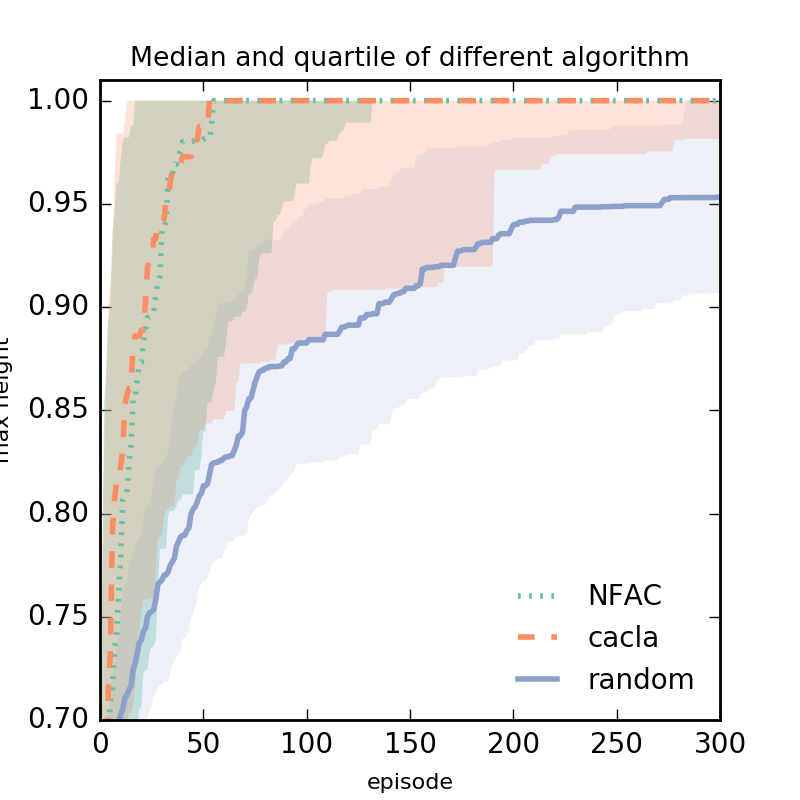
\includegraphics{result_plotting/adacrobot-1ddl.png}
		\caption{..}
		\label{image:adacrobot}
	\end{center}
\end{figure}
Median performance of cacla and NFAC are equivalent. However NFAC is more stable as the lower quartile reach the max performance
at episode 150 where 300 is needed with cacla.

Statistics have been made over 150 different runs after meta-parameters optimization for each algorithms.

\DRAFT{
\begin{itemize}
 \item Acrobot 1DDL
 \begin{itemize}
  \item Cacla
  \item NFAC
 \end{itemize}
 
 \item Cartpole
  \begin{itemize}
  \item Cacla
  \item NFAC
 \end{itemize}
\end{itemize}
}